\PassOptionsToPackage{usenames}{color}
\documentclass[11pt,letterpaper]{article}
%\usepackage[a4paper,margin=1in]{geometry}

\usepackage{relsize} % relative font sizes (e.g. \smaller). must precede ACL style
\usepackage{naaclhlt2015}
\usepackage[colorlinks=true,linkcolor=black,citecolor=black,filecolor=black,urlcolor=black]{hyperref}
\usepackage{natbib}

%\usepackage{times}
%\usepackage{latexsym}

\usepackage{microtype}

\usepackage[boxed]{algorithm2e}
\renewcommand\AlCapFnt{\small}
\usepackage[small,bf,skip=5pt]{caption}
\usepackage{sidecap} % side captions
\usepackage{rotating}	% sideways

% Italicize subparagraph headings
\usepackage{titlesec}
\titleformat*{\section}{\large\larger[.5]\bfseries}
\titleformat*{\subsection}{\large\bfseries}
\titleformat*{\subsubsection}{\large\bfseries}
\titleformat*{\paragraph}{\large\bfseries}
\titleformat*{\subparagraph}{\itshape}
\titlespacing{\subparagraph}{%
  1em}{%              left margin
  0pt}{% space before (vertical)
  1em}%               space after (horizontal)

% Numbered Examples and lists
\usepackage{lingmacros}

\usepackage{enumitem} % customizable lists
\setitemize{noitemsep,topsep=0em}
\setenumerate{noitemsep,leftmargin=0em,itemindent=13pt,topsep=0em}


\usepackage{textcomp}
% \usepackage{arabtex} % must go after xparse, if xparse is used!
%\usepackage{utf8}
% \setcode{utf8} % use UTF-8 Arabic
% \newcommand{\Ar}[1]{\RL{\novocalize #1}} % Arabic text

\usepackage{listings}

\lstset{
  basicstyle=\itshape,
  xleftmargin=3em,
  aboveskip=0pt,
  belowskip=-3pt, %-.5\baselineskip, % correct for extra paragraph break inserted after listing
  literate={->}{$\rightarrow$}{2}
           {α}{$\alpha$}{1}
           {δ}{$\delta$}{1}
           {(}{$($}{1}
           {)}{$)$}{1}
           {[}{$[$}{1}
           {]}{$]$}{1}
           {|}{$|$}{1}
           {+}{\ensuremath{^+}}{1}
           {*}{\ensuremath{^*}}{1}
}

\usepackage{amssymb}	%amsfonts,eucal,amsbsy,amsthm,amsopn
\usepackage{amsmath}

\usepackage{mathptmx}	% txfonts
\usepackage[scaled=.8]{beramono}
\usepackage[T1]{fontenc}
\usepackage[utf8x]{inputenc}

\usepackage{MnSymbol}	% must be after mathptmx

\usepackage{latexsym}





% Tables
\usepackage{array}
\usepackage{multirow}
\usepackage{booktabs} % pretty tables
\usepackage{wrapfig}
\usepackage{multicol}
\usepackage{footnote}

\usepackage{url}
\usepackage[usenames]{color}
\usepackage{xcolor}

% colored frame box
\newcommand{\cfbox}[2]{%
    \colorlet{currentcolor}{.}%
    {\color{#1}%
    \fbox{\color{currentcolor}#2}}%
}

\usepackage[normalem]{ulem} % \uline
\usepackage{colortbl}
\usepackage{graphicx}
\usepackage{subcaption}
%\usepackage{tikz-dependency}
\usepackage{tikz}
%\usepackage{tree-dvips}
\usetikzlibrary{arrows,positioning,calc} 

\DeclareMathOperator*{\argmax}{arg\,max}
\DeclareMathOperator*{\argmin}{arg\,min}
%\setlength\titlebox{6.5cm}    % Expanding the titlebox



% Author comments
\usepackage{color}
\newcommand\bmmax{0} % magic to avoid 'too many math alphabets' error
\usepackage{bm}
\definecolor{orange}{rgb}{1,0.5,0}
\definecolor{mdgreen}{rgb}{0,0.6,0}
\definecolor{mdblue}{rgb}{0,0,0.7}
\definecolor{dkblue}{rgb}{0,0,0.5}
\definecolor{dkgray}{rgb}{0.3,0.3,0.3}
\definecolor{slate}{rgb}{0.25,0.25,0.4}
\definecolor{gray}{rgb}{0.5,0.5,0.5}
\definecolor{ltgray}{rgb}{0.7,0.7,0.7}
\definecolor{purple}{rgb}{0.7,0,1.0}
\definecolor{lavender}{rgb}{0.65,0.55,1.0}

% Settings for algorithm listings
% \lstset{
%   language=Python,
%   upquote=true,
%   showstringspaces=false,
%   formfeed=\newpage,
%   tabsize=1,
%   commentstyle=\itshape\color{lavender},
%   basicstyle=\small\smaller\ttfamily,
%   morekeywords={lambda},
%   emph={upward,downward,tc},
%   emphstyle=\underbar,
%   aboveskip=0cm,
%   belowskip=-.5cm
% }
%\renewcommand{\lstlistingname}{Algorithm}


\newcommand{\ensuretext}[1]{#1}
\newcommand{\jmfmarker}{\ensuretext{\textcolor{green}{\ensuremath{^{\textsc{JM}}_{\textsc{F}}}}}}
\newcommand{\cjdmarker}{\ensuretext{\textcolor{blue}{\ensuremath{^{\textsc{CJ}}_{\textsc{D}}}}}}
\newcommand{\nssmarker}{\ensuretext{\textcolor{magenta}{\ensuremath{^{\textsc{NS}}_{\textsc{S}}}}}}
\newcommand{\nasmarker}{\ensuretext{\textcolor{red}{\ensuremath{^{\textsc{NA}}_{\textsc{S}}}}}}
\newcommand{\jbmarker}{\ensuretext{\textcolor{orange}{\ensuremath{^{\textsc{J}}_{\textsc{B}}}}}}
\newcommand{\dbmarker}{\ensuretext{\textcolor{purple}{\ensuremath{^{\textsc{D}}_{\textsc{B}}}}}}
\newcommand{\arkcomment}[3]{\ensuretext{\textcolor{#3}{[#1 #2]}}}
%\newcommand{\arkcomment}[3]{}
\newcommand{\jmf}[1]{\arkcomment{\jmfmarker}{#1}{green}}
\newcommand{\cjd}[1]{\arkcomment{\cjdmarker}{#1}{blue}}
\newcommand{\nss}[1]{\arkcomment{\nssmarker}{#1}{magenta}}
\newcommand{\nas}[1]{\arkcomment{\nasmarker}{#1}{red}}
\newcommand{\jb}[1]{\arkcomment{\jbmarker}{#1}{orange}}
\newcommand{\db}[1]{\arkcomment{\dbmarker}{#1}{purple}}
\newcommand{\wts}{\mathbf{w}}
\newcommand{\g}{\mathbf{g}}
\newcommand{\f}{\mathbf{f}}
\newcommand{\x}{\mathbf{x}}
\newcommand{\y}{\mathbf{y}}
\newcommand{\overbar}[1]{\mkern 1.5mu\overline{\mkern-1.5mu#1\mkern-1.5mu}\mkern 1.5mu} % \bar is too narrow in math
\newcommand{\cost}{c}

\newcommand{\Sref}[1]{\S\ref{#1}}
\newcommand{\fref}[1]{figure~\ref{#1}}
\newcommand{\ffref}[2]{figures~\ref{#1} and~\ref{#2}}
\newcommand{\Fref}[1]{Figure~\ref{#1}}
\newcommand{\FFref}[2]{Figures~\ref{#1} and~\ref{#2}}
\newcommand{\tref}[1]{table~\ref{#1}}
\newcommand{\ttref}[2]{tables~\ref{#1} and~\ref{#2}}
\newcommand{\Tref}[1]{Table~\ref{#1}}
\newcommand{\aref}[1]{algorithm~\ref{#1}}
\newcommand{\Aref}[1]{Algorithm~\ref{#1}}
\newcommand{\fnref}[1]{footnote~\ref{#1}}

\newcommand{\citeposs}[2][]{\citeauthor{#2}'s (\citeyear[#1]{#2})}
\newcommand{\Citeposs}[2][]{\Citeauthor{#2}'s (\citeyear[#1]{#2})}


% Space savers
% From http://www.eng.cam.ac.uk/help/tpl/textprocessing/squeeze.html
% \addtolength{\dbltextfloatsep}{-.5cm} % space between last top float or first bottom float and the text.
% \addtolength{\intextsep}{-.5cm} % space left on top and bottom of an in-text float.
% \addtolength{\abovedisplayskip}{-.5cm} % space before maths
% \addtolength{\belowdisplayskip}{-.5cm} % space after maths
% %\addtolength{\topsep}{-.5cm} %space between first item and preceding paragraph
% \setlength{\belowcaptionskip}{-.25cm}


% customize \paragraph spacing
\makeatletter
\renewcommand{\paragraph}{%
  \@startsection{paragraph}{4}%
  {\z@}{.2ex \@plus 1ex \@minus .2ex}{-1em}%
  {\normalfont\normalsize\bfseries}%
}
\makeatother



% Special macros
\newcommand{\tg}[1]{\texttt{#1}}	% supersense tag name
\newcommand{\gfl}[1]{%\renewcommand\texttildelow{{\lower.74ex\hbox{\texttt{\char`\~}}}} % http://latex.knobs-dials.com/
\mbox{\textsmaller{\texttt{#1}}}}	% supersense tag symbol
\newcommand{\lex}[1]{\textsmaller{\textsf{\textcolor{slate}{\textbf{#1}}}}}	% example lexical item 
\newcommand{\tagdef}[1]{#1\hfill} % tag definition
\newcommand{\tagt}[2]{\ensuremath{\underset{\textrm{\textlarger{\tg{#2}}}\strut}{\w{#1}\rule[-.3\baselineskip]{0pt}{0pt}}}} % tag text (a word or phrase) with an SST. (second arg is the tag)
\newcommand{\glosst}[2]{\ensuremath{\underset{\textrm{#2}}{\textrm{#1}}}} % gloss text (a word or phrase) (second arg is the gloss)
\newcommand{\AnnA}[0]{\mbox{\textbf{Ann-A}}} % annotator A
\newcommand{\AnnB}[0]{\mbox{\textbf{Ann-B}}} % annotator B
\newcommand{\sys}[1]{\mbox{\textbf{#1}}}   % name of a system (one of our experimental conditions)
\newcommand{\dataset}[1]{\mbox{\textsc{#1}}}	% one of the datasets in our experiments
\newcommand{\datasplit}[1]{\mbox{\textbf{#1}}}	% portion one of the datasets in our experiments

\newcommand{\w}[1]{\textit{#1}}	% word
\newcommand{\gap}[0]{\ \ } % space around gap contents
\newcommand{\tat}[0]{\textasciitilde}

\newcommand{\shortlong}[2]{#1} % short vs. long version of the paper
\newcommand{\confversion}[1]{#1}
\newcommand{\srsversion}[1]{}
\newcommand{\finalversion}[1]{#1}
%\newcommand{\finalversion}[1]{}
\newcommand{\shortversion}[1]{#1}
\newcommand{\considercutting}[1]{#1}
\newcommand{\longversion}[1]{} % ...if only there were more space...
\newcommand{\subversion}[1]{#1} % for the submission version only
\newcommand{\draftnotice}[1]{} % for the draft version only
%\newcommand{\subversion}[1]{}

\hyphenation{WordNet}
\hyphenation{WordNets}
\hyphenation{VerbNet}
\hyphenation{FrameNet}
\hyphenation{SemCor}
\hyphenation{PennConverter}
\hyphenation{an-aly-sis}
\hyphenation{an-aly-ses}
\hyphenation{news-text}
\hyphenation{base-line}
\hyphenation{de-ve-lop-ed}
\hyphenation{comb-over}

\title{The Logic of AMR: Practical, Unified, Graph-Based\\ Sentence Semantics for NLP}

\author{Nathan Schneider\\
	University of Edinburgh\\
	{\tt nschneid@inf.ed.ac.uk}
\And
	Jeffrey Flanigan\\
	Carnegie Mellon University\\
	{\tt jflanigan@cs.cmu.edu}
	    }

% \author{Author 1\\
% 	    XYZ Company\\
% 	    111 Anywhere Street\\
% 	    Mytown, NY 10000, USA\\
% 	    {\tt author1@xyz.org}
% 	  \And
% 	Author 2\\
%   	ABC University\\
%   	900 Main Street\\
%   	Ourcity, PQ, Canada A1A 1T2\\
%   {\tt author2@abc.ca}}

\date{}

\begin{document}
\maketitle

\begin{abstract}
This tutorial will offer a detailed introduction to the Abstract Meaning Representation (AMR) formalism 
and its use for sentence semantics in NLP. Our goals are twofold. 
First, we will describe the nature and design principles behind the representation, 
and demonstrate that it can be practical for annotation. Participants will be coached in the basics of annotation 
so they will be prepared to work with existing data with an understanding of the benefits and limitations 
of the process by which it was created. 
Second, we will survey the state of the art for computation with AMRs. 
This will focus on the task of parsing English text into AMR graphs, which 
requires algorithms for alignment, for structured prediction, and for statistical learning. 
Advances toward AMR-based machine translation and other multilingual studies\nss{vague} will be reviewed as well.
\end{abstract}

\section{Introduction}

The Abstract Meaning Representation formalism \citep[AMR;][]{amr} 
is rapidly emerging as an important practical form of structured sentence semantics. 
Conceived just a few years ago, AMR has enjoyed momentum thanks to 
the ongoing development of large-scale annotated corpora 
(20k sentences annotated; an additional 45k expected by the end of 2015).
It has stimulated research in automata-theoretic formalisms \citep{jones-12,chiang-13}
as well as structured prediction algorithms \citep{flanigan-14}.
Following on the heels of the Fred Jelinek Memorial Workshop in Prague (summer, 2014), 
which explored the cross-lingual linguistic and computational implications of AMR, 
this tutorial unmasks the design philosophy, data creation process, and existing algorithms for 
AMR semantics.

The proposed tutorial structure is in two main parts. 
Roughly speaking, the first half will be devoted to linguistic and annotation matters, 
while the second half will focus on algorithms and applications.
By the end of the first half, participants will have a firm grasp of the AMR representation, 
which will help motivate the technical challenges of the second half.

Below, we give an extremely brief description of how AMR works and why it has potential 
as a convergence point\nss{?} for NLP research. 
That will be followed by a high-level overview of the tutorial goals and structure, 
as well as a tentative schedule.

\section{Why AMR?}


\jmf{when we talk about the tutorial's goals and structure, we could mention that we'll briefly review structured prediction and discriminative training}

\begin{figure*}\centering
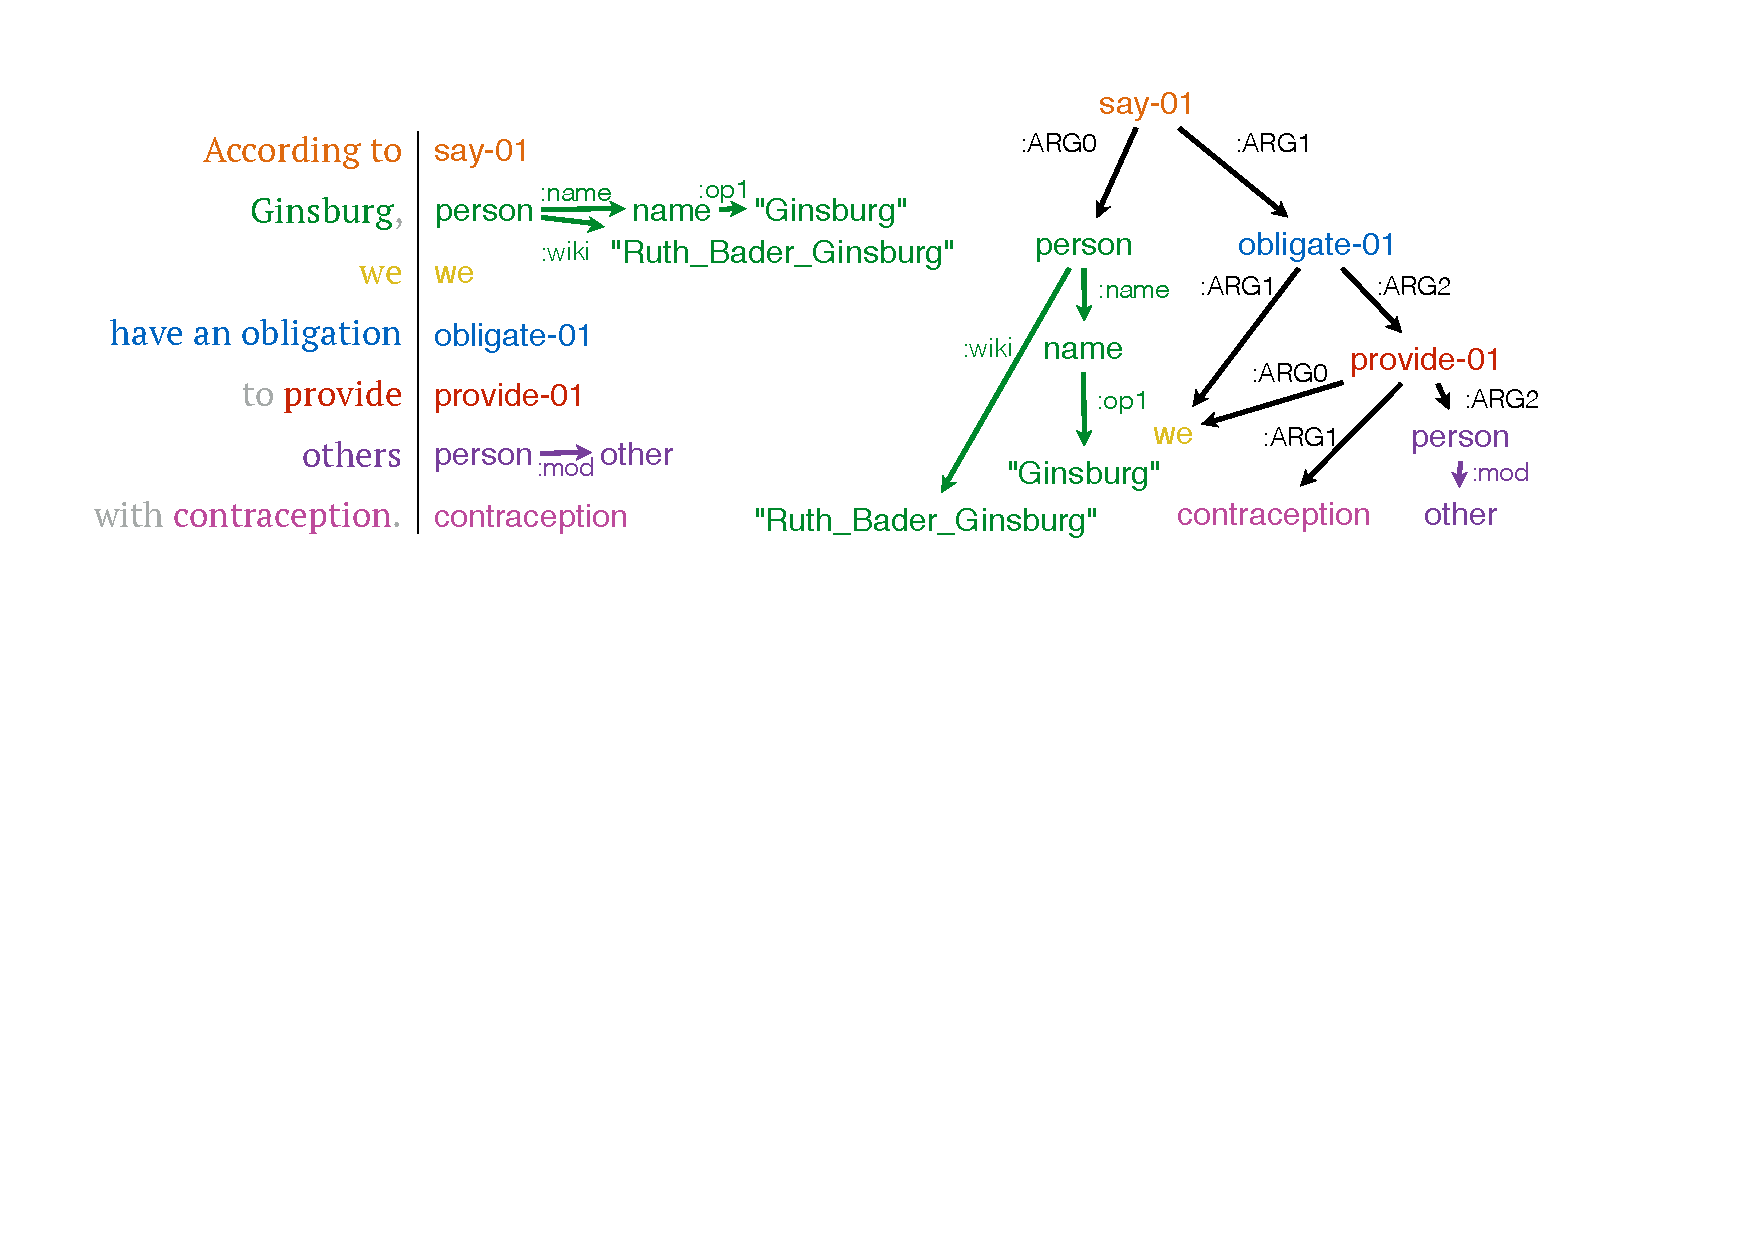
\includegraphics[width=.87\textwidth]{ginsburg.pdf}
\caption{A sentence from a political blog (left) and its AMR graph (right). 
Between them are fragments of the graph that would ideally be aligned to fragments of the sentence. 
Near-paraphrases like \textit{Ginsburg said that we will be obligated to provide contraception to other people.}\ 
would receive the same AMR.}
\label{fig:ginsburg}
\end{figure*}


The need for an abstract meaning representation to disambiguate linguistic utterances, 
to expose meaning overlaps between utterances, and to mediate between multiple languages 
was recognized in the era of interlingua-based MT \citep{dorr-98}. 
The contemporary AMR reimagines such a formalism in light of the successes of data-driven NLP.
Crucially, it was designed from the start for large-scale annotation. 
In the interest of practicality, therefore, it establishes conventions for how different elements 
of meaning are to be abstractly represented; necessarily, some elements are given a deeper treatment 
than others, and a few grammatical devices (including tense, aspect, number, and definiteness) 
are treated as external to the representation.
\Citeposs{amr} AMR is envisioned not as a new start for computational semantics, 
but rather as a point of contact for bread-and-butter NLP tasks---%
sense disambiguation and semantic role labeling for predicates in PropBank \citep{propbank,bonial-14}; 
named entity recognition; nominal relation identification; 
coreference resolution and entity linking---which are usually approached in isolation. 
At the same time, it draws attention to certain semantic analysis problems that have been 
acknowledged but largely neglected, such as modality identification \citep{prabhakaran-12}.
AMR brings these NLP tasks under the umbrella of a single full-sentence semantics, 
with a single evaluation. The example in \fref{fig:ginsburg} illustrates many of these components.

Most of the advances in AMR thus far have been in formalizing the representation, 
creating a large (and growing) corpus,\footnote{The AMR Bank, comprising 
public data from \textit{The Little Prince} (\url{http://amr.isi.edu/download.html}) 
and an LDC general release of sentences from ``newswire, weblogs and web discussion forums'' \citep{amr-ldc}.} 
and working out how to predict AMRs for English sentences. 
We expect that these developments will soon lead to applications 
involving multilinguality, machine translation, paraphrasing, and summarization.

\begin{figure}\centering
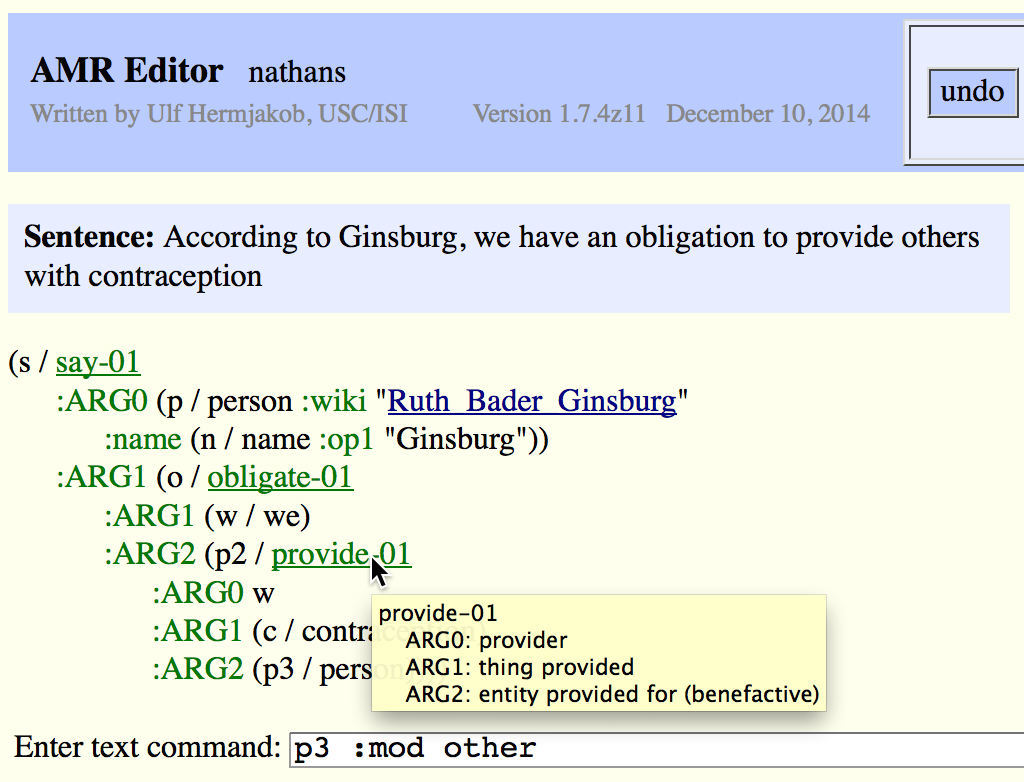
\includegraphics[width=\columnwidth]{editor_zoomed.png}
\caption{Ulf Hermjakob's AMR Editor for annotation includes a command line for fast entry and manipulation of AMRs, 
predicate documentation from PropBank, a query tool for finding existing AMRs, automatic consistency-checking heuristics, 
and extensive documentation of AMR conventions.}
\label{fig:editor}
\end{figure}

\section{Agenda}

Our primary topics will be English AMR annotation and parsing. 
We will also give an overview (in less depth) of some promising theoretical and applied directions 
that have been explored in preliminary work, but do not yet have empirical results.

\begin{enumerate}
\item The AMR formalism for English \begin{itemize}
	\item How meaning is structured (20\%)
	\item What is not represented, and how AMR differs from alternatives (10\%)
	\item Annotation tools and data resources (5\%)
	\item Guided annotation practice with the AMR Editor (15\%)
	\end{itemize}
\item Algorithms and applications \begin{itemize}
	\item AMR alignment, parsing, and evaluation (30\%)
	\item Multilinguality, machine translation, and other applications (15\%)
	\item Open challenges, criticisms, and limitations (5\%)
	\end{itemize}
\end{enumerate}
\jmf{this list looks good to me, does it need to be more fine-grained? I could try to break the time down more precisely.}

\section{Logistics}

The authors will hold dry runs of the tutorial at their respective institutions, 
which will be especially important for debugging the hands-on activities. 

\nss{venue; attendance; equipment required}
\jmf{internet connection for people's laptops}

\section{Instructors}

\textbf{Nathan Schneider} (\url{http://nathan.cl}) is an annotation schemer and computational modeler for natural language. 
He has been involved in the design of the AMR formalism since 2012, 
when he interned with Kevin Knight at ISI. 
His dissertation introduced a coarse-grained representation for lexical semantics that facilitates rapid annotation 
and is practical for broad-coverage statistical NLP \citep{schneider-thesis}. 
He has also worked on semantic parsing for the FrameNet representation \citep{das-14} 
and other forms of annotation and processing for social media text \citep{gimpel-11,owoputi-13,schneider-13,kong-14,mohit-12}.
For most of these projects, he led the design of the annotation scheme, guidelines, and workflows, 
and the training and supervision of annotators.
He will lead the first half of the tutorial.\\[-5pt]

\noindent \textbf{Jeffrey Flanigan} (\url{http://www.cs.cmu.edu/~jmflanig/}) is a fifth year Ph.D. candidate at Carnegie Mellon University.
He and his collaborators at CMU built the first broad-coverage AMR parser \citep{flanigan-14}.
He also participated in the Fred Jelinek Memorial Workshop in Prague in 2014, working on cross-lingual parsing and generation from AMR.
His research areas include machine translation, summarization, and semantic dependency parsing.
He will lead the second half of the tutorial.

\bibliographystyle{aclnat}
% you bib file should really go here
\setlength{\bibsep}{1pt}
{\fontsize{10}{12.25}\selectfont
\bibliography{amr}}

\end{document}
